\documentclass[12pt]{article}

\usepackage{fullpage}
\usepackage{graphicx, rotating, booktabs} 
\usepackage{times} 
\usepackage{natbib} 
\usepackage{indentfirst} 
\usepackage{setspace}
\usepackage{grffile} 
\usepackage{hyperref}
\usepackage{adjustbox}
\setcitestyle{aysep{}}


\singlespace
\title{\textbf{Appendix to Paper: Alliance Participation, Treaty Depth and Military Spending}}
%\author{Joshua Alley}
\date{}

\bibliographystyle{apsr}

\begin{document}

\maketitle 

\doublespace 



\section{Priors}

\autoref{tab:priors} summarizes the prior distributions in the multilevel model. 
All priors are weakly informative relative to the scale of the data. 
$\nu$ is the degrees of freedom for the t-distribution, and the gamma prior is the recommended default prior for STAN. 

\begin{table} % Create a table of priors.
\begin{center}
\begin{tabular}{c} 
$ p(\alpha) \sim N(0, 1)$  \\
$ p(\sigma) \sim \mbox{half-}N(0, 1) $ \\
$ p(\alpha^{yr}) \sim N(0, \sigma^{yr}) $ \\ 
$ p(\sigma^{yr}) \sim N(0, 1) $ \\
$ p(\alpha^{st}) \sim N(0, \sigma^{st}) $ \\ 
$ p(\sigma^{st}) \sim \mbox{half-}N(0, .5) $ \\ 
$ p(\sigma^{all}) \sim \mbox{half-}N(0, .5) $ \\
$ p(\beta) \sim N(0, .5) $ \\
$ p(\gamma) \sim N(0, .5) $ \\ 
$ p(\nu) \sim gamma(2, 0.1)$ 
\end{tabular} 
\caption{Summary of Priors in Multilevel Model} 
\label{tab:priors}
\end{center} 
\end{table} 


\section{Hamiltonian Monte Carlo Diagnostics}

There were no divergent iterations in either sample running 4 chains for 2,000 iterations with 1,000 warmup iterations. 
The $\hat{R}$ is less than 1.1 for all parameters in both samples. 
Trace plots in \autoref{fig:trace-all-min} indicate good mixing of the chains for the alliance-level parameters. 
Taken together, all of this implies that the chains adequately explored the posterior distribution. 

\begin{figure}[htbp]
	\centering
		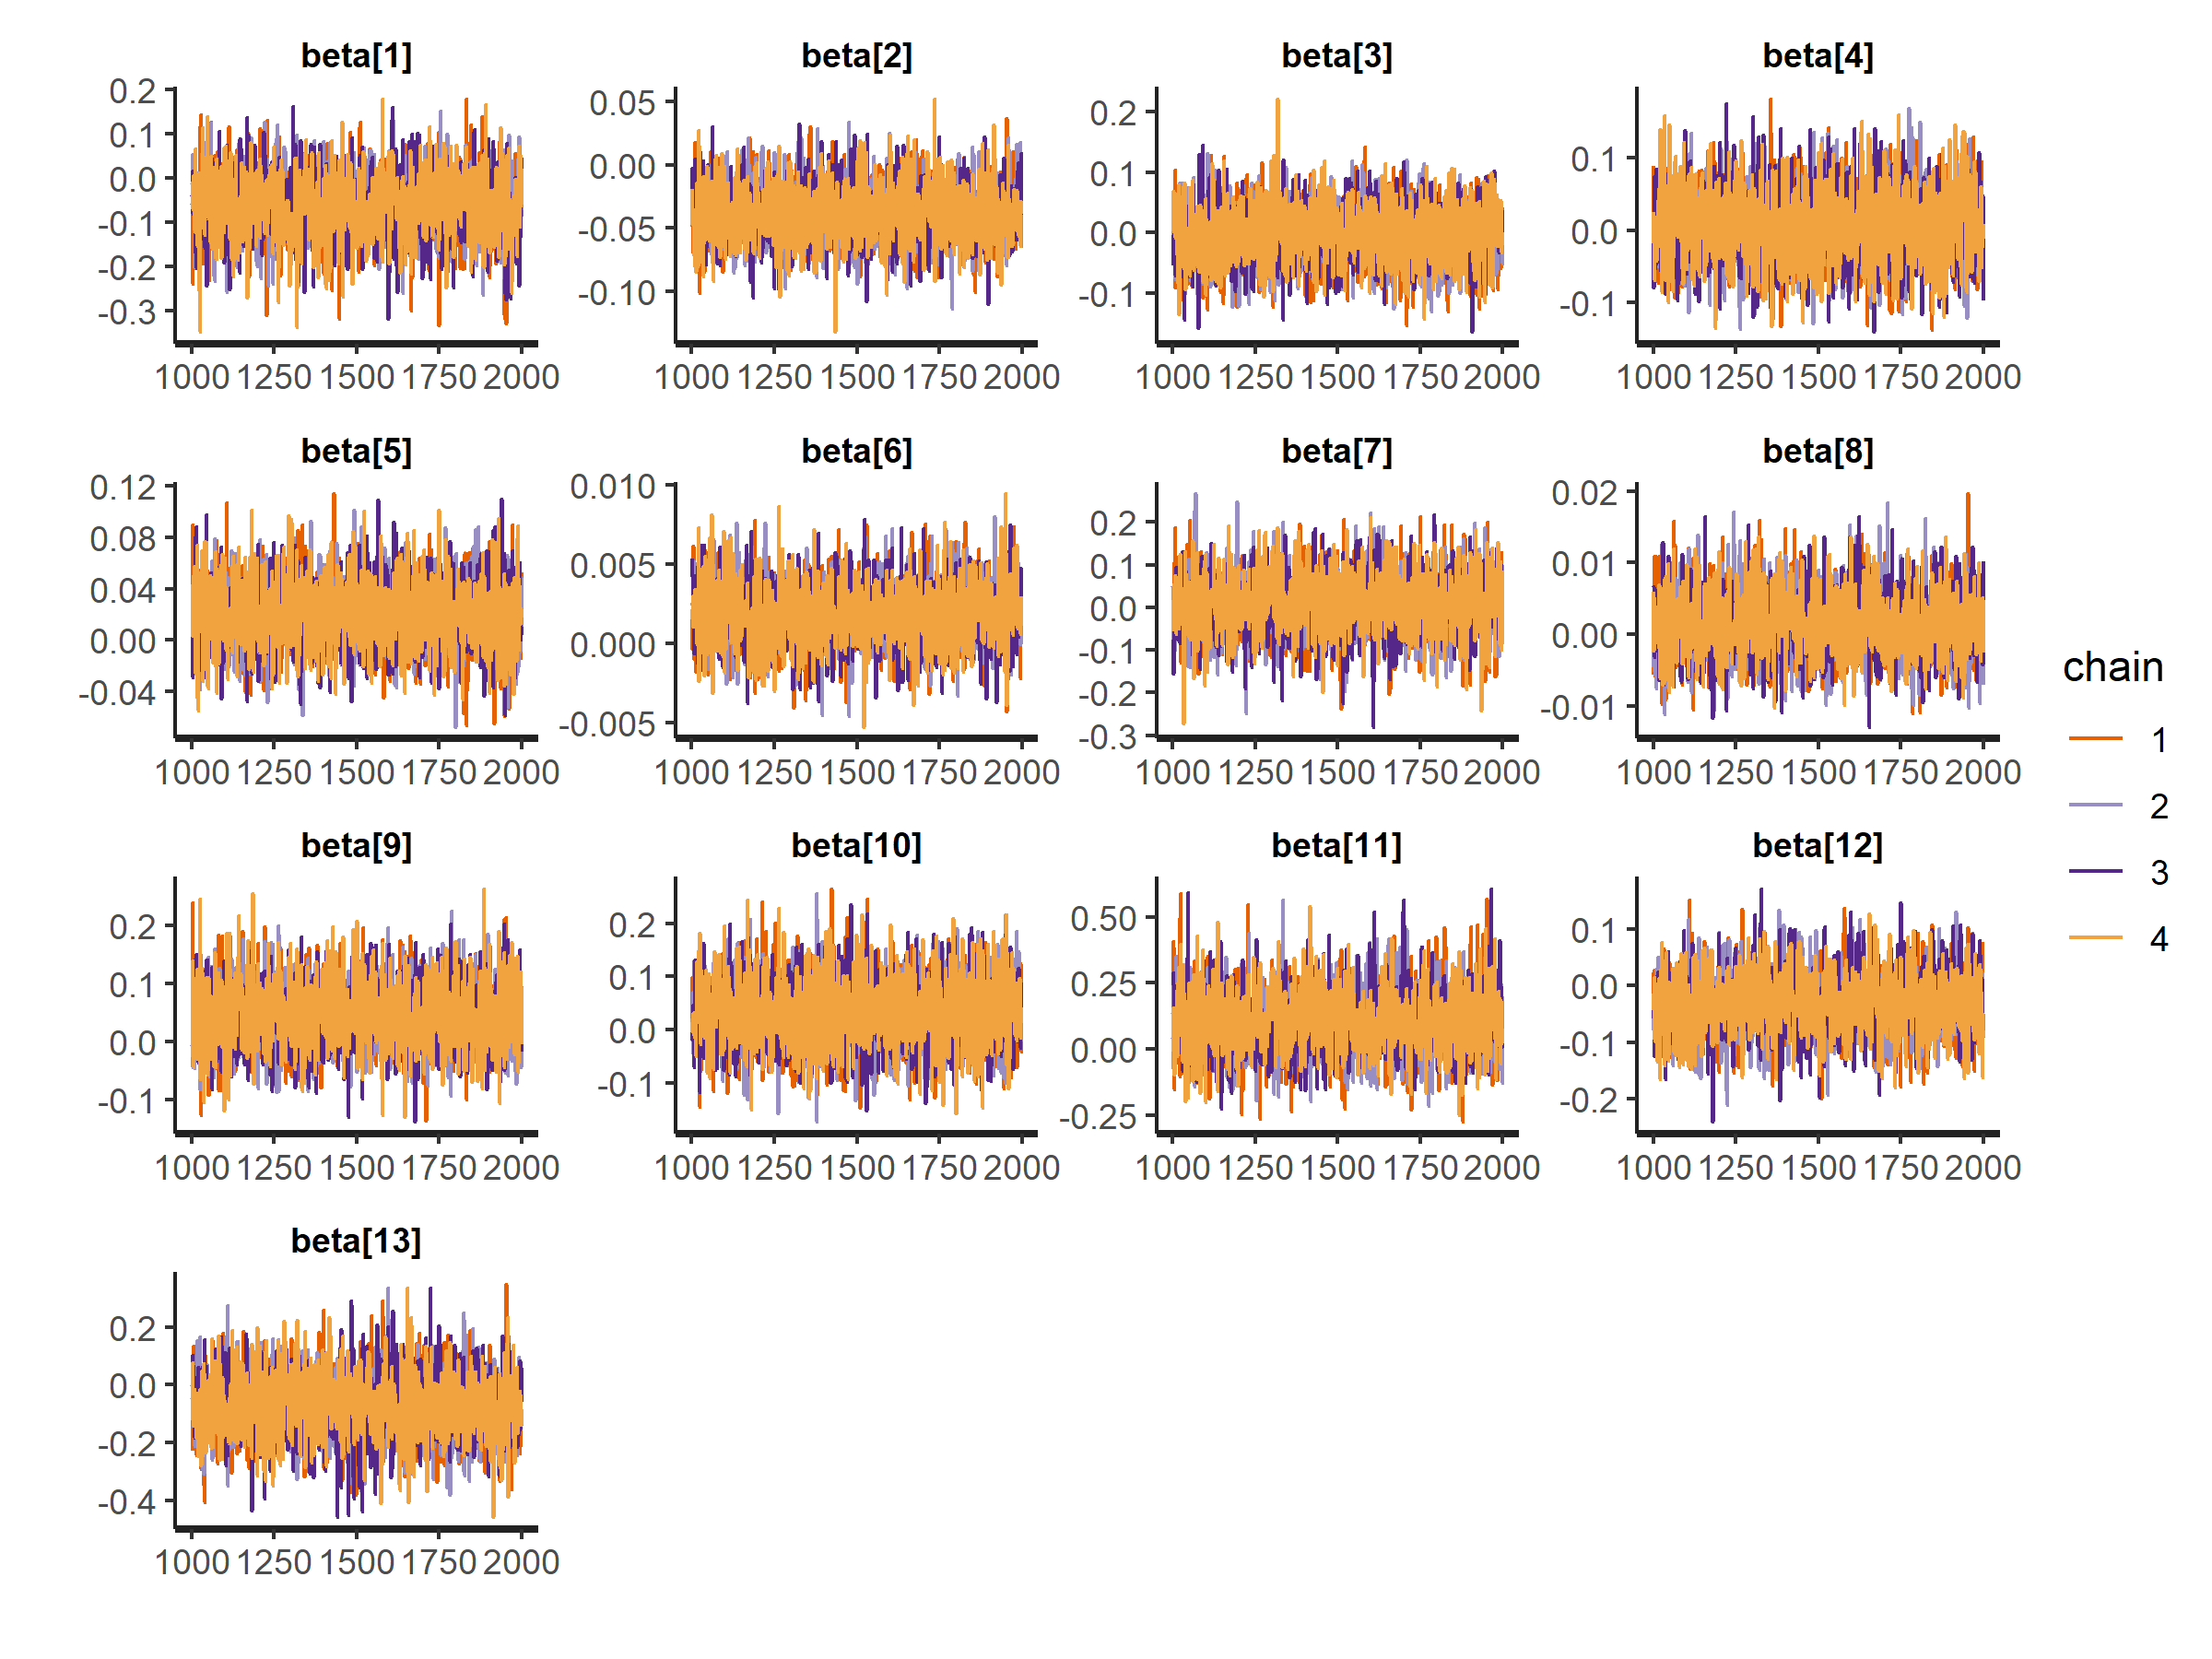
\includegraphics[width=0.95\textwidth]{trace-all-min.png}
	\caption{Traceplot of alliance level parameters in the non-major power sample.}
	\label{fig:trace-all-min}
\end{figure}



\section{Fake Data Simulation Check}


With any complicated model, simulating fake data and seeing if the model can recover known parameters is an essential check. 
Fake-data simulation helps validate model results. 
This section summarizes results from fitting the multilevel model to fake data.


I simulated a dataset of 2000 t-distributed observations with 50 states observed for 200 years and 100 alliances. 
The outcome has a different scale than the military spending growth variable in the paper.
Thus coefficient values here will not match reported values in the paper.  
I then simulated two state and alliance level variables and a sparse matrix of state membership in alliances. 
Last, I ran the model without evaluating the likelihood, generating a posterior prediction of the outcome based on the fake data.


To check whether the model could recover known parameters, I took the 12th draw of the posterior distribution.
This draw included a simulated outcome for each observation and a set of coefficients. 
I then fit the multilevel model on the simulated outcome values and checked whether the credible intervals contained the corresponding parameter values. 
If a parameter is within the 90\% credible interval, the model captures it. 


The model recovers known parameters with a high degree of accuracy. 
As shown by \autoref{fig:beta-sim-res}, the two credible intervals of the alliance-level regression include the known values.
Credible interval coverage for the variance hyperparameters and $\gamma$ parameters is also acceptable. 


\begin{figure}[htbp]
	\centering
		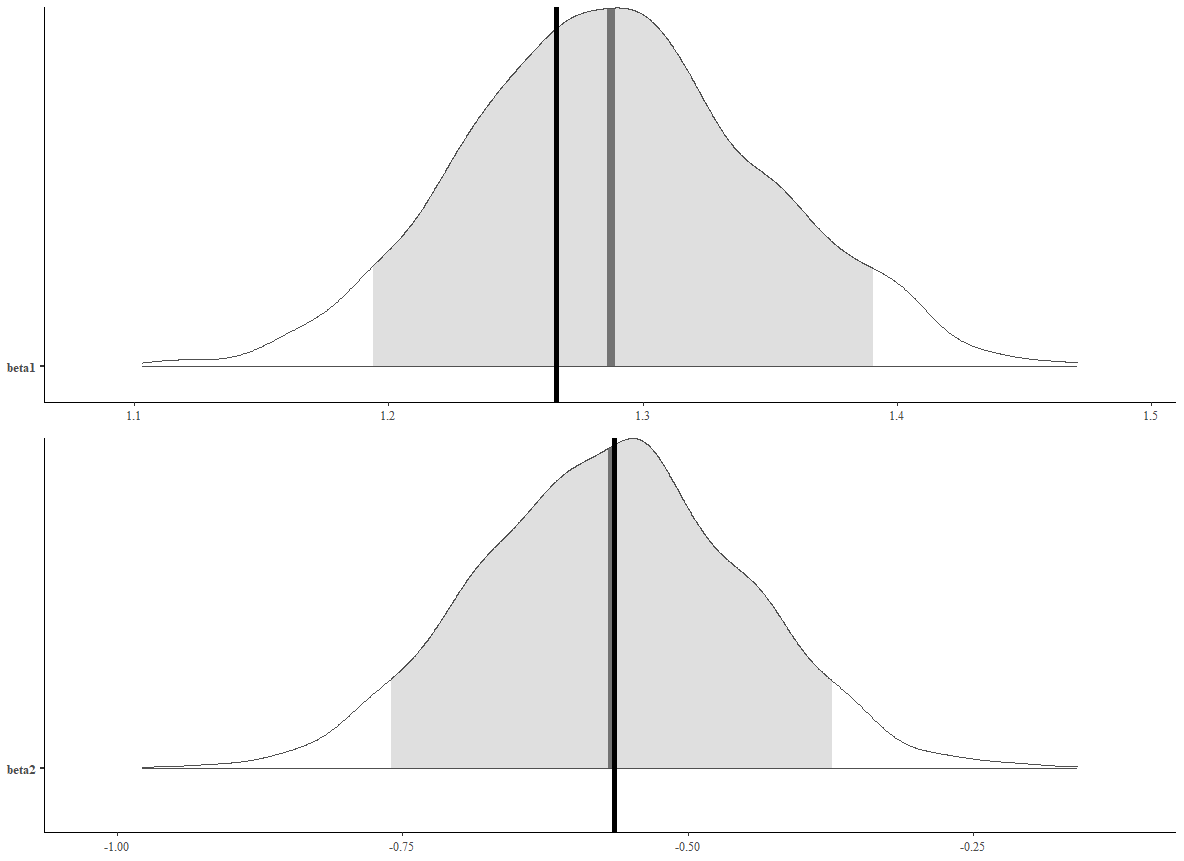
\includegraphics[width=0.95\textwidth]{beta-sim-res.png}
	\caption{Posterior distributions of $\beta$ parameters from fitting multilevel model to fake data. The black vertical line marks the known parameter value, and the grey area is the 90\% credible interval.}
	\label{fig:beta-sim-res}
\end{figure}


 
Even with small multiples, the 100 $\lambda$ parameters are harder to plot, so I offer a descriptive summary here. 
Among the $\lambda$ parameters, 93 of 100 intervals contain the known $\lambda$ value.
Given the large number of parameters and smaller sample, this is acceptable accuracy. 
Even the seven inaccurate confidence intervals were quite close--- all were within .015 of the known parameter.\footnote{Fine margins around these intervals implies that the exact number of accurate $\lambda$ intervals is sensitive to simulation variance.}


In summary, convergence diagnostics and fake data fitting both suggest that the multilevel model is working well. 
No convergence diagnostics indicate problems exploring the posterior. 
Just as importantly, the model can recover known parameters from fake data. 
The next section provides more detail on results from the major and non-major power samples. 



\section{Posterior Intervals} 


I do not present tabular summaries of the alliance-level parameters in the manuscript. 
The next table summarizes the posteriors of the alliance-level parameters. 
Using a 90\% credible intervals implies there is a 90\% chance the coefficient is between the 5\% and 95\% values. 
Because Hypotheses 1 is directional, I report the negative posterior probability in the manuscript.  
Like a one-tailed hypothesis test, the positive and negative posterior probabilities match the hypotheses better. 


\autoref{tab:alliance-level-min} summarize the 90\% credible intervals for the alliance-level regression parameters in the non-major power sample. 
The $\hat{R}$ statistics are all close to one, indicating convergence. 
The number of effective samples is adequate for all parameters.

\begin{table}[ht]
\centering
\begin{tabular}{rrrrrrr}
  \hline
 & Mean & S.D. & 5\% & 95\% & Num. Eff. & $\hat{R}$ \\ 
  \hline
Constant & -0.03 & 0.03 & -0.08 & 0.02 & 1677.92 & 1.00 \\ 
  Depth & 0.02 & 0.02 & -0.00 & 0.05 & 2521.36 & 1.00 \\ 
  Econ. Link & -0.02 & 0.02 & -0.04 & 0.01 & 2997.70 & 1.00 \\ 
  FP Conc. & 0.01 & 0.01 & -0.00 & 0.03 & 4019.10 & 1.00 \\ 
  Number Members & 0.00 & 0.00 & -0.00 & 0.00 & 3820.06 & 1.00 \\ 
  FP Similarity & 0.00 & 0.03 & -0.04 & 0.05 & 2254.34 & 1.00 \\ 
  Democratic Membership & -0.00 & 0.00 & -0.00 & 0.00 & 4412.89 & 1.00 \\ 
  Wartime & 0.04 & 0.03 & -0.01 & 0.08 & 3474.44 & 1.00 \\ 
  Asymmetric & -0.03 & 0.02 & -0.07 & 0.01 & 3474.45 & 1.00 \\ 
  US. Mem & 0.02 & 0.02 & -0.01 & 0.05 & 2330.47 & 1.00 \\ 
  USSR Mem. & 0.04 & 0.05 & -0.03 & 0.12 & 3859.50 & 1.00 \\ 
  $\sigma$ Alliances & 0.02 & 0.01 & 0.00 & 0.03 & 1201.91 & 1.01 \\ 
   \hline
\end{tabular}
\caption{90\% Credible intervals non-major power alliance-level parameters}
\label{tab:alliance-level-min}
\end{table}



\section{Robustness Check: Single-Level Regression}

Though the multilevel model best reflects the theory, I find similar results with single-level models. 
In what follows, I briefly present results from robust regressions of state-year growth in military spending. 
In these models, the key independent variable is the average depth of a state's alliances. 
This compares states as the depth of their alliance portfolio shifts. 
In addition to the state-level controls in the multilevel model, I included averages of alliance size and democracy and the log of total allied capability as controls. 


I estimated several models, including robust regressions on all states, non-major powers, and non-major powers in alliances. 
I also applied fixed effects to an OLS model of growth in defense expenditures. 
The estimated association between average treaty depth and military spending growth is summarized in \autoref{fig:single-level-mplot}. 
In all four models, average treaty depth has a positive and statistically significant association with spending growth in one-tailed tests. 


\begin{figure}[htbp]
	\centering
		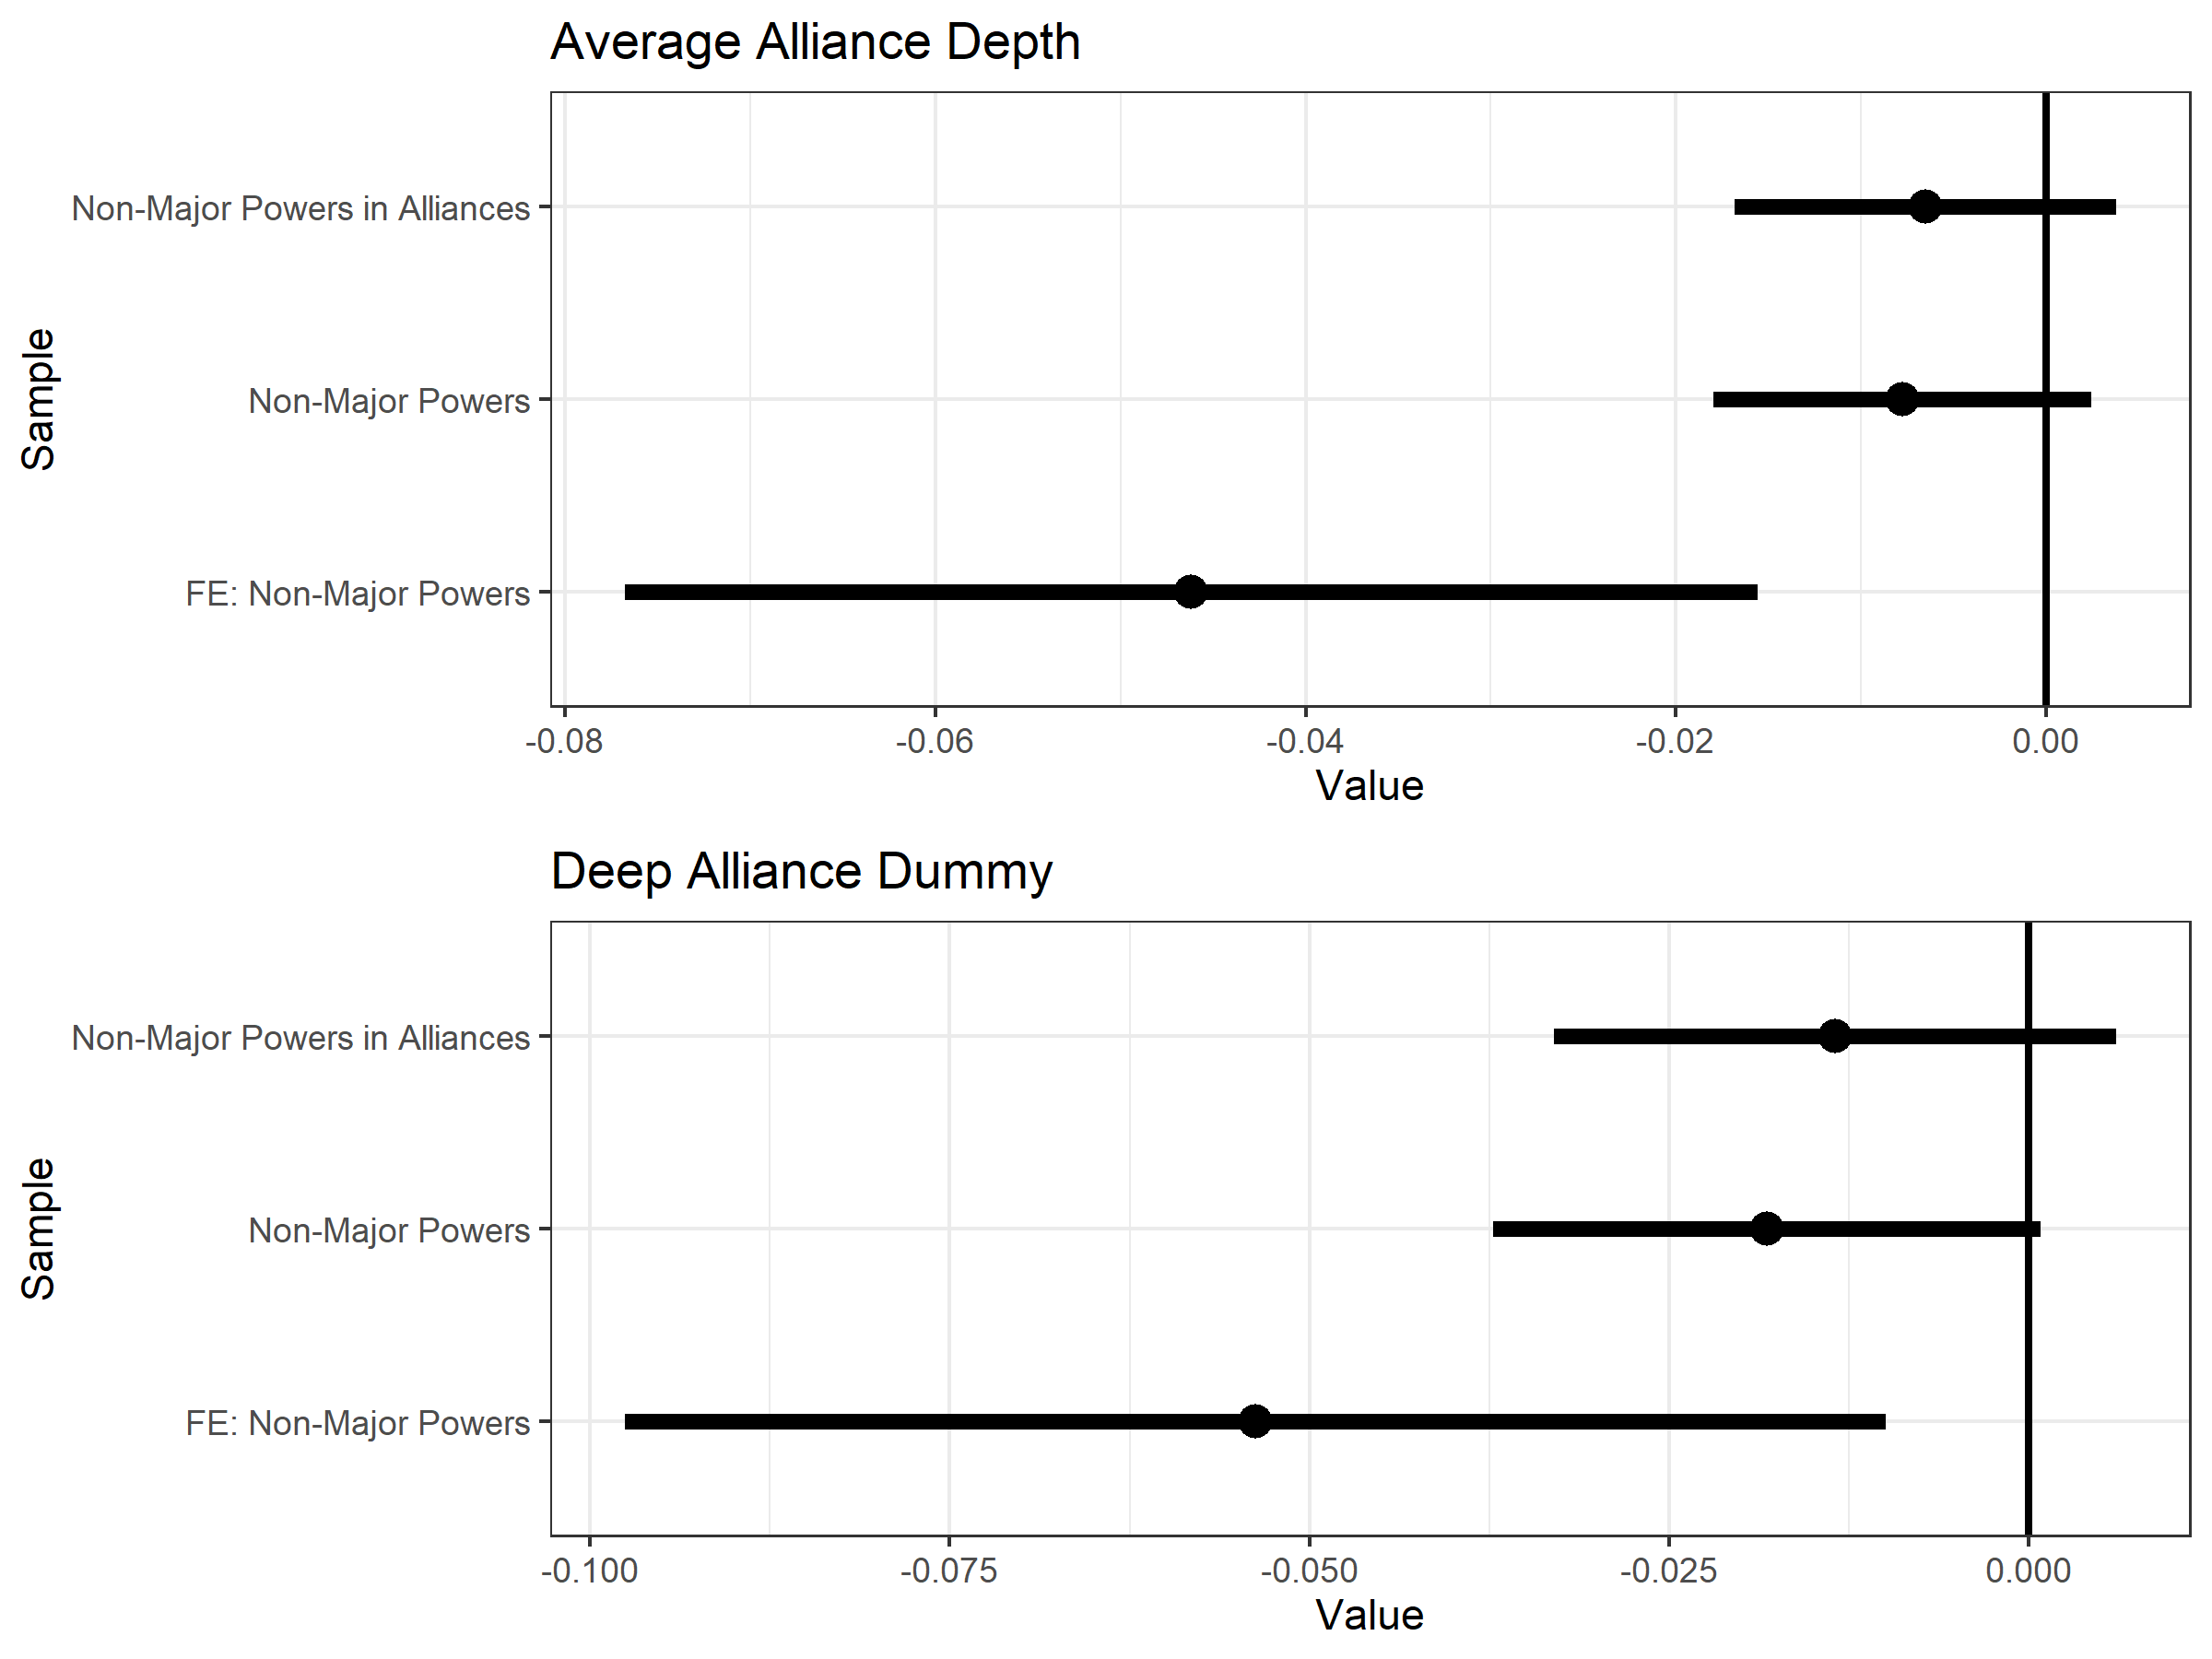
\includegraphics[width=0.95\textwidth]{single-level-mplot.png}
	\caption{Estimated effect of average alliance treaty depth on growth in military spending }
	\label{fig:single-level-mplot}
\end{figure}


The analysis of non-major powers in alliances is the best approximation of the multilevel model, as it compares non-major powers with different kinds of alliances. 
Analyzing a sample of all non-major powers includes states with no alliances, with does not match the comparison in the multilevel model. 
To assess the robustness of the coefficient estimate in the sample of non-major powers with alliances, I performed Extreme Bounds analysis. 
Specifically, I present results from \citet{Sala-i-Martin1997}'s method of bounds analysis in \autoref{fig:eba-single-level}. 


\autoref{fig:eba-single-level} shows the distribution of the average treaty depth coefficient and an indicator of whether the alliance includes economic agreements. 
Across many specifications, where all regression coefficients are doubtful, the CDF of the average depth coefficient has 98\% positive mass. 
Even though the normality assumption is tenuous, the histogram in \autoref{fig:eba-single-level} shows little evidence increases in treaty depth reduce growth in military spending. 
The bounds analysis indicates average treaty depth is a robust predictor of growth in military spending across over 1500 possible specifications. 


\begin{figure}[htbp]
	\centering
		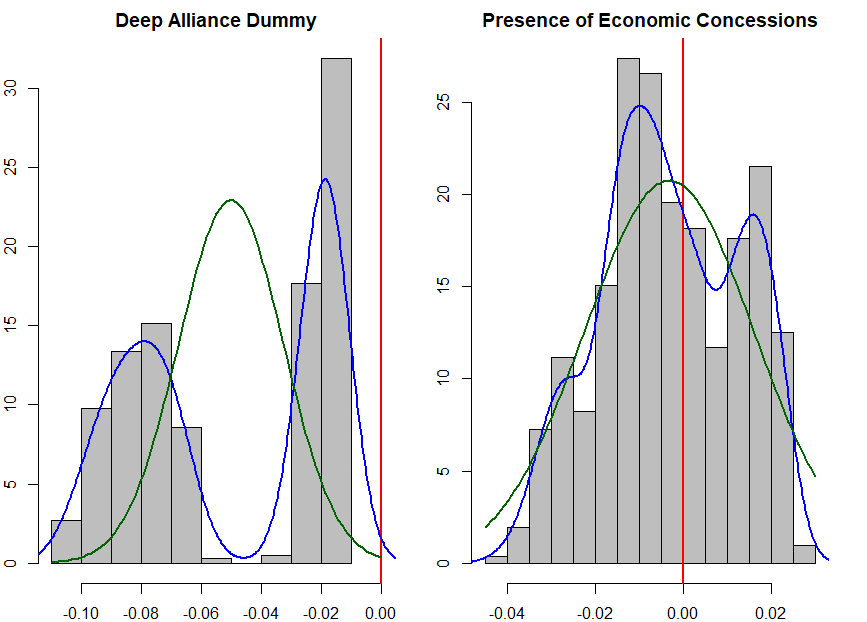
\includegraphics[width=0.95\textwidth]{eba-single-level.png}
	\caption{Histogram of regression}
	\label{fig:eba-single-level}
\end{figure}



  
\bibliography{../../MasterBibliography} 




\end{document}
